\documentclass[onlymath]{beamer}
% \documentclass[onlymath,handout]{beamer}

% Macros used by all lectures, but not necessarily by excercises

%%% General setup and dependencies:

% \usetheme[ddcfooter,nosectionnum]{tud}
\usetheme[nosectionnum,pagenum,noheader]{tud}
% \usetheme[nosectionnum,pagenum]{tud}

% Increase body font size to a sane level:
\let\origframetitle\frametitle
% \renewcommand{\frametitle}[1]{\origframetitle{#1}\normalsize}
\renewcommand{\frametitle}[1]{\origframetitle{#1}\fontsize{10pt}{13.2}\selectfont}
\setbeamerfont{itemize/enumerate subbody}{size=\small} % tud defaults to scriptsize!
\setbeamerfont{itemize/enumerate subsubbody}{size=\small}
% \setbeamerfont{normal text}{size=\small}
% \setbeamerfont{itemize body}{size=\small}

\renewcommand{\emph}[1]{\textbf{#1}}

\def\arraystretch{1.3}% Make tables even less cramped vertically

\usepackage[ngerman]{babel}
\usepackage[utf8]{inputenc}
\usepackage[T1]{fontenc}

%\usepackage{graphicx}
\usepackage[export]{adjustbox} % loads graphicx
\usepackage{import}
\usepackage{stmaryrd}
\usepackage[normalem]{ulem} % sout command
% \usepackage{times}
\usepackage{txfonts}
\usepackage{array}

% \usepackage[perpage]{footmisc} % reset footnote counter on each page -- fails with beamer (footnotes gone)
\usepackage{perpage}  % reset footnote counter on each page
\MakePerPage{footnote}

\usepackage{tikz}
\usetikzlibrary{arrows,positioning,decorations.pathreplacing}
% Inspired by http://www.texample.net/tikz/examples/hand-drawn-lines/
\usetikzlibrary{decorations.pathmorphing}
\pgfdeclaredecoration{penciline}{initial}{
    \state{initial}[width=+\pgfdecoratedinputsegmentremainingdistance,
    auto corner on length=1mm,]{
        \pgfpathcurveto%
        {% From
            \pgfqpoint{\pgfdecoratedinputsegmentremainingdistance}
                      {\pgfdecorationsegmentamplitude}
        }
        {%  Control 1
        \pgfmathrand
        \pgfpointadd{\pgfqpoint{\pgfdecoratedinputsegmentremainingdistance}{0pt}}
                    {\pgfqpoint{-\pgfdecorationsegmentaspect
                     \pgfdecoratedinputsegmentremainingdistance}%
                               {\pgfmathresult\pgfdecorationsegmentamplitude}
                    }
        }
        {%TO
        \pgfpointadd{\pgfpointdecoratedinputsegmentlast}{\pgfpoint{1pt}{1pt}}
        }
    }
    \state{final}{}
}
\tikzset{handdrawn/.style={decorate,decoration=penciline}}
\tikzset{every shadow/.style={fill=none,shadow xshift=0pt,shadow yshift=0pt}}
% \tikzset{module/.append style={top color=\col,bottom color=\col}}

% Use to make Tikz attributes with Beamer overlays
% http://tex.stackexchange.com/a/6155
\tikzset{onslide/.code args={<#1>#2}{%
  \only<#1| handout:0>{\pgfkeysalso{#2}}
}}
\tikzset{onslideprint/.code args={<#1>#2}{%
  \only<#1>{\pgfkeysalso{#2}}
}}

%%% Title -- always set this first

\newcommand{\defineTitle}[3]{
	\newcommand{\lectureindex}{#1}
	\title{Theoretische Informatik und Logik}
	\subtitle{\href{\lectureurl}{#1. Vorlesung: #2}}
	\author{\href{https://iccl.inf.tu-dresden.de/web/Markus_Kr\%C3\%B6tzsch}{Markus Kr\"{o}tzsch}\\[1ex]Lehrstuhl Wissensbasierte Systeme}
	\date{#3}
	\datecity{TU Dresden}
% 	\institute{CC-By 3.0, sofern keine anderslautenden Bildrechte angegeben sind}
}

%%% Table of contents:

\RequirePackage{ifthen}

\newcommand{\highlight}[2]{%
	\ifthenelse{\equal{#1}{\lectureindex}}{\alert{#2}}{#2}%
}

\def\myspace{-0.7ex}
\newcommand{\printtoc}{
\begin{tabular}{r@{$\quad$}l}
\highlight{1}{1.} & \highlight{1}{Willkommen/Einleitung formale Sprachen}\\[\myspace]
\highlight{2}{2.} & \highlight{2}{Grammatiken und die Chomsky-Hierarchie}\\[\myspace]
\highlight{3}{3.} & \highlight{3}{Endliche Automaten}\\[\myspace]
\highlight{4}{4.} & \highlight{4}{Complexity of FO query answering}\\[\myspace]
\highlight{5}{5.} & \highlight{5}{Conjunctive queries}\\[\myspace]
\highlight{6}{6.} & \highlight{6}{Tree-like conjunctive queries}\\[\myspace]
\highlight{7}{7.} & \highlight{7}{Query optimisation}\\[\myspace]
\highlight{8}{8.} & \highlight{8}{Conjunctive Query Optimisation / First-Order~Expressiveness}\\[\myspace]
\highlight{9}{9.} & \highlight{9}{First-Order~Expressiveness / Introduction to Datalog}\\[\myspace]
\highlight{10}{10.} & \highlight{10}{Expressive Power and Complexity of Datalog}\\[\myspace]
\highlight{11}{11.} & \highlight{11}{Optimisation and Evaluation of Datalog}\\[\myspace]
\highlight{12}{12.} & \highlight{12}{Evaluation of Datalog (2)}\\[\myspace]
\highlight{13}{13.} & \highlight{13}{Graph Databases and Path Queries}\\[\myspace]
\highlight{14}{14.} & \highlight{14}{Outlook: database theory in practice}
\end{tabular}
}

\newcommand{\overviewslide}{%
\begin{frame}\frametitle{Overview}
\printtoc
\medskip

Siehe \href{\lectureurl}{course homepage [$\Rightarrow$ link]} for more information and materials
\end{frame}
}

%%% Colours:
\usepackage{xcolor,colortbl}
\definecolor{redhighlights}{HTML}{FFAA66}
\definecolor{lightblue}{HTML}{55AAFF}
\definecolor{lightred}{HTML}{FF5522}
\definecolor{lightpurple}{HTML}{DD77BB}
\definecolor{lightgreen}{HTML}{55FF55}
\definecolor{darkred}{HTML}{CC4411}
\definecolor{darkblue}{HTML}{176FC0}%{1133AA}
\definecolor{nightblue}{HTML}{2010A0}%{1133AA}
\definecolor{alert}{HTML}{176FC0}
\definecolor{darkgreen}{HTML}{36AB14}
\definecolor{strongyellow}{HTML}{FFE219}
\definecolor{devilscss}{HTML}{666666}

\newcommand{\redalert}[1]{\textcolor{darkred}{#1}}

%%% Slide layout commands:

\newcommand{\sectionSlide}[1]{
\frame{\begin{center}
\LARGE
#1
\end{center}}
}
\newcommand{\sectionSlideNoHandout}[1]{
\frame<handout:0>{\begin{center}
\LARGE
#1
\end{center}}
}

\newcommand{\mydualbox}[3]{%
 \begin{minipage}[t]{#1}
 \begin{beamerboxesrounded}[upper=block title,lower=block body,shadow=true]%
    {\centering\usebeamerfont*{block title}#2}%
    \raggedright%
    \usebeamerfont{block body}
%     \small
    #3%
  \end{beamerboxesrounded}
  \end{minipage}
}
%
\newcommand{\myheaderbox}[2]{%
 \begin{minipage}[t]{#1}
 \begin{beamerboxesrounded}[upper=block title,lower=block title,shadow=true]%
    {\centering\usebeamerfont*{block title}\rule{0pt}{2.6ex} #2}%
  \end{beamerboxesrounded}
  \end{minipage}
}

\newcommand{\mycontentbox}[2]{%
 \begin{minipage}[t]{#1}%
 \begin{beamerboxesrounded}[upper=block body,lower=block body,shadow=true]%
    {\centering\usebeamerfont*{block body}\rule{0pt}{2.6ex}#2}%
  \end{beamerboxesrounded}
  \end{minipage}
}

\newcommand{\mylcontentbox}[2]{%
 \begin{minipage}[t]{#1}%
 \begin{beamerboxesrounded}[upper=block body,lower=block body,shadow=true]%
    {\flushleft\usebeamerfont*{block body}\rule{0pt}{2.6ex}#2}%
  \end{beamerboxesrounded}
  \end{minipage}
}

% label=180:{\rotatebox{90}{{\footnotesize\textcolor{darkgreen}{Beispiel}}}}
% \hspace{-8mm}\ghost{\raisebox{-7mm}{\rotatebox{90}{{\footnotesize\textcolor{darkgreen}{Beispiel}}}}}\hspace{8mm}
\newcommand{\examplebox}[1]{%
	\begin{tikzpicture}[decoration=penciline, decorate]
		\pgfmathsetseed{1235}
		\node (n1) [decorate,draw=darkgreen, fill=darkgreen!10,thick,align=left,text width=\linewidth, inner ysep=2mm, inner xsep=2mm] at (0,0) {#1};
% 		\node (n2) [align=left,text width=\linewidth,inner sep=0mm] at (n1.92) {{\footnotesize\raisebox{3mm}{\textcolor{darkgreen}{Beispiel}}}};
% 		\node (n2) [decorate,draw=darkgreen, fill=darkgreen!10,thick, align=left,text width=\linewidth,inner sep=2mm] at (n1.90) {{\footnotesize\raisebox{0mm}{\textcolor{darkgreen}{Beispiel}}}};
	\end{tikzpicture}%
}%

\newcommand{\codebox}[1]{%
	\begin{tikzpicture}[decoration=penciline, decorate]
		\pgfmathsetseed{1236}
		\node (n1) [decorate,draw=strongyellow, fill=strongyellow!10,thick,align=left,text width=\linewidth, inner ysep=2mm, inner xsep=2mm] at (0,0) {#1};
	\end{tikzpicture}%
}%

\newcommand{\defbox}[1]{%
	\begin{tikzpicture}[decoration=penciline, decorate]
		\pgfmathsetseed{1237}
		\node (n1) [decorate,draw=darkred, fill=darkred!10,thick,align=left,text width=\linewidth, inner ysep=2mm, inner xsep=2mm] at (0,0) {#1};
	\end{tikzpicture}%
}%

\newcommand{\theobox}[1]{%
	\begin{tikzpicture}[decoration=penciline, decorate]
		\pgfmathsetseed{1240}
		\node (n1) [decorate,draw=darkblue, fill=darkblue!10,thick,align=left,text width=\linewidth, inner ysep=2mm, inner xsep=2mm] at (0,0) {#1};
	\end{tikzpicture}%
}%

\newcommand{\anybox}[2]{%
	\begin{tikzpicture}[decoration=penciline, decorate]
		\pgfmathsetseed{1240}
		\node (n1) [decorate,draw=#1, fill=#1!10,thick,align=left,text width=\linewidth, inner ysep=2mm, inner xsep=2mm] at (0,0) {#2};
	\end{tikzpicture}%
}%


\newsavebox{\mybox}%
\newcommand{\doodlebox}[2]{%
\sbox{\mybox}{#2}%
	\begin{tikzpicture}[decoration=penciline, decorate]
		\pgfmathsetseed{1238}
		\node (n1) [decorate,draw=#1, fill=#1!10,thick,align=left,inner sep=1mm] at (0,0) {\usebox{\mybox}};
	\end{tikzpicture}%
}%


\defineTitle{5}{Der Satz von Rice und das Postsche Korrespondenzproblem}{21. April 2017}

\begin{document}

\maketitle


\begin{frame}\frametitle{Wesentliche Ergebnisse bisher}

\emph{Viele Dinge sind nicht berechenbar:}
\begin{itemize}
\item Die Busy-Beaver-Funktion
\item Das Halteproblem
\item Das $\epsilon$-Halteproblem
\end{itemize}
\bigskip

\emph{Dazu gibt es mehrere Beweismethoden:}
\begin{itemize}
\item \alert{Kardinalitätsargumente:} Anzahl Algorithmen vs. Anzahl Probleme
\item \alert{Diagonalisierungen:} Nimm Berechenbarkeit an und konstruiere damit (als Subroutine) einen paradoxen Algorithmus
\item \alert{Reduktionen:} Zeige, dass bereits bekannte nicht berechenbare Probleme sich lösen liesen, wenn das Problem berechenbar wäre
\end{itemize}

\end{frame}


\begin{frame}\frametitle{Der Satz von Rice}

Ein interessantes Resultat von Henry Gordon Rice bewahrt uns davor, noch hunderte andere Probleme im Detail zu betrachten:\medskip

\theobox{Satz von Rice (informelle Version): Jede nicht-triviale Frage über die von einer TM ausgeführte Berechnung ist unentscheidbar.}\bigskip\pause

\theobox{Satz von Rice (formell): Sei $E$ eine Eigenschaft von Sprachen, die für manche Turing-erkennbare Sprachen gilt und für manche Turing-erkennbare Sprachen nicht gilt (="`nicht-triviale Eigenschaft"'). Dann ist das folgende Problem unentscheidbar:
\begin{itemize}
\item Eingabe: Turingmaschine $\Smach{M}$
\item Ausgabe: Hat $\Slang{L}(\Smach{M})$ die Eigenschaft $E$?
\end{itemize}}


\end{frame}

\begin{frame}\frametitle{Alles unentscheidbar}

\examplebox{Beispiele für Fragen, die laut Rice unentscheidbar sind:
\begin{itemize}
\item "`Ist $\Sterm{aba}\in\Slang{L}(\Smach{M})$?"' 
\item "`Ist $\Slang{L}(\Smach{M})$ leer?"'
\item "`Ist $\Slang{L}(\Smach{M})$ endlich?"'
\item "`Ist $\Slang{L}(\Smach{M})$ regulär?"'
\item \ldots
\end{itemize}
Rice ist dagegen nicht anwendbar auf:
\begin{itemize}
\item "`Hat $\Smach{M}$ mindestens zwei Zustände?"'\\ (keine Eigenschaft von $\Slang{L}(\Smach{M})$) 
\item "`Ist $\Slang{L}(\Smach{M})$ semi-entscheibar?"' (trivial)
\item \ldots
\end{itemize}
}

Der Satz von Rice lässt sich sinngemäß auf alle Turing-mächtigen Formalismen übertragen.

\end{frame}

\begin{frame}[t]\frametitle{Der Satz von Rice: Beweis (1)}

\theobox{Satz von Rice: Sei $E$ eine nicht-triviale Eigenschaft von Turing-erkennbaren Sprachen. Dann ist das folgende unentscheidbar:%
\begin{itemize}
\item Eingabe: Turingmaschine $\Smach{M}$
\item Ausgabe: Hat die Sprache $\Slang{L}(\Smach{M})$ die Eigenschaft $E$?
\end{itemize}}

\emph{Beweis:} Sei $E$ eine Eigenschaft wie im Satz. Wir konstruieren eine
Many-One-Reduktion vom $\epsilon$-Halteproblem auf "`$E$-Haftigkeit"'.\bigskip

\begin{itemize}
\item Sei $\emptyset\notin E$ 
	(o.b.d.A.: wir könnten sonst auch Unentscheidbarkeit von $\overline{E}$ beweisen)
\item Sei $\Smach{M}_{\Slang{L}}$ eine TM, die eine Sprache $\Slang{L}\in E$ akzeptiert\\
	(muss existieren, da $E$ nicht-trivial ist)
% \item Sei $\Smach{M}_\emptyset$ eine TM mit $\Slang{L}(\Smach{M}_\emptyset)=\emptyset$
%%% <- Könnte man als Wert für falsch kodierte Eingaben nutzen, aber das ist nicht nötig
\end{itemize}

\end{frame}

\begin{frame}[t]\frametitle{Der Satz von Rice: Beweis (2)}

\theobox{Satz von Rice: Sei $E$ eine nicht-triviale Eigenschaft von Turing-erkennbaren Sprachen. Dann ist das folgende unentscheidbar:%
\begin{itemize}
\item Eingabe: Turingmaschine $\Smach{M}$
\item Ausgabe: Hat die Sprache $\Slang{L}(\Smach{M})$ die Eigenschaft $E$?
\end{itemize}}

\emph{Beweis (Fortsetzung):}\pause{} 
Für eine beliebige TM $\Smach{M}$ sei $\Smach{M}^*$ eine TM, die für eine Eingabe
$w$ das folgende tut:
\begin{enumerate}[(1)]
\item Simuliere $\Smach{M}$ auf dem leeren Wort $\epsilon$
\item Falls $\Smach{M}$ hält, simuliere $\Smach{M}_{\Slang{L}}$ auf $w$
\end{enumerate}\medskip\pause
Damit gilt: falls $\Smach{M}$ auf $\epsilon$ hält, dann $\Slang{L}(\Smach{M}^*)=\Slang{L}\in E$ und\\
\mbox{}\phantom{Damit gilt:} falls $\Smach{M}$ auf $\epsilon$ nicht hält, dann $\Slang{L}(\Smach{M}^*)=\emptyset\notin E$
\medskip\pause

Eine geeignete Many-One-Reduktion $f$ ist demnach:
\[f(v)=\left\{\begin{array}{ll}
\textsf{enc}(\Smach{M}^*) & \text{falls $v=\textsf{enc}(\Smach{M})$ für eine TM $\Smach{M}$}\\
\Sterm{\#} & \text{falls die Eingabe nicht korrekt kodiert ist $\quad$\qed}
\end{array}\right.\]

\end{frame}


\sectionSlide{Semi-Entscheidbarkeit}

\begin{frame}\frametitle{Das Halteproblem, schon wieder}

Wir haben gesehen, dass das Halteproblem unentscheidbar ist,
aber es ist dennoch Turing-erkennbar:\bigskip

\theobox{Satz: Das Halteproblem ist semi-entscheidbar.}

\pause\emph{Beweis:} Eine Turingmaschine, die das Halteproblem erkennt, ist
leicht skizziert:
\begin{itemize}
\item Wenn die Eingabe die Form $\textsf{enc}(\Smach{M})\#\#\textsf{enc}(w)$ hat
\item dann simuliere $\Smach{M}$ auf Eingabe $w$.
\item Wenn $\Smach{M}$ hält, dann halte und akzeptiere.\qed
\end{itemize}

Im Wesentlichen ist die TM für das Halteproblem also die universelle Turingmaschine.

\end{frame}

\begin{frame}\frametitle{Komplementierung}

\emph{Rückblick (Vorlesung Formale Systeme):} Für eine Sprache $\Slang{L}$ bezeichnet $\overline{\Slang{L}}$ die \alert{Komplementsprache}:
\[ \overline{\Slang{L}} = \{w\in\Sigma^*\mid w\notin\Slang{L} \}\]\pause

\theobox{Satz: Für jede Sprache $\Slang{L}$ gibt es Turing-Reduktionen $\overline{\Slang{L}}\leq_T\Slang{L}$ und $\Slang{L}\leq_T\overline{\Slang{L}}$.}

\pause
\emph{Beweis:} Der Algorithmus für die Reduktion $\overline{\Slang{L}}\leq_T\Slang{L}$ ist sehr einfach:
\begin{itemize}
\item Für Eingabe $w$,
\item entscheide zunächst ob $w\in\Slang{L}$
\item und invertiere das Ergebnis anschließend.
\end{itemize}
Die Umkehrung $\Slang{L}\leq_T\overline{\Slang{L}}$ funktioniert ebenso.\qed
\bigskip\pause

\theobox{Korrolar: $\Slang{L}$ ist genau dann entscheidbar, wenn $\overline{\Slang{L}}$ entscheidbar ist.}

\end{frame}

\begin{frame}[t]\frametitle{Zwei halbe Entscheidbarkeiten = eine ganze}

Es gibt einen interessanten Zusammenhang von Komplementierung und Semi-Entscheidbarkeit:\\[1ex]

\theobox{Satz: $\Slang{L}$ ist genau dann entscheidbar, wenn $\Slang{L}$ und $\overline{\Slang{L}}$ semi-entscheibar sind.
}\pause

\emph{Beweis:} "`$\Rightarrow$"' Angenommen $\Slang{L}$ ist entscheidbar.\pause

\begin{itemize}
\item Dann ist $\Slang{L}$ per Definition auch semi-entscheidbar.
\item Außerdem ist auch $\overline{\Slang{L}}$ entscheidbar (gerade gezeigt), also ebenfalls semi-entscheidbar.
\end{itemize}

\end{frame}

\begin{frame}[t]\frametitle{Zwei halbe Entscheidbarkeiten = eine ganze}

Es gibt einen interessanten Zusammenhang von Komplementierung und Semi-Entscheidbarkeit:\\[1ex]

\theobox{Satz: $\Slang{L}$ ist genau dann entscheidbar, wenn $\Slang{L}$ und $\overline{\Slang{L}}$ semi-entscheibar sind.
}

\emph{Beweis:} "`$\Leftarrow$"' Wenn $\Slang{L}$ und $\overline{\Slang{L}}$ semi-entscheibar sind, dann werden sie durch TMs $\Smach{M}_{\Slang{L}}$ und
$\Smach{M}_{\overline{\Slang{L}}}$ erkannt.\pause\medskip

Algorithmus: Für Eingabe $w$, iteriere über alle $n=1,2,3,\ldots$
\begin{itemize}
\item Simuliere $\Smach{M}_{\Slang{L}}$ für $n$ Schritte:\\
	Wenn $\Smach{M}_{\Slang{L}}$ akzeptiert, dann halte und akzeptiere
\item Simuliere $\Smach{M}_{\overline{\Slang{L}}}$ für $n$ Schritte:\\
	Wenn $\Smach{M}_{\overline{\Slang{L}}}$ akzeptiert, dann halte und verwerfe
\item Ansonsten fahre mit nächstem $n$ fort.
\end{itemize}
Dieser Algorithmus ist korrekt und terminiert für jede Eingabe, da immer
entweder $\Smach{M}_{\Slang{L}}$ oder
$\Smach{M}_{\overline{\Slang{L}}}$ terminieren muss.\qed

\end{frame}

\begin{frame}\frametitle{Co-Semi-Entscheidbarkeit}

Wir können unsere Einsichten zusammenfassen:\bigskip

\theobox{Korrolar: Wenn $\Slang{L}$ unentscheidbar aber semi-entscheidbar ist, dann
kann $\overline{\Slang{L}}$ nicht semi-entscheidbar (und auch nicht entscheidbar) sein.
}\bigskip\pause

\examplebox{Beispiel: Sei $\overline{\Slang{P}}_{\textsf{Halt}}$ das Komplement des
Halteproblems $\Slang{P}_{\textsf{Halt}}$. Dann ist $\overline{\Slang{P}}_{\textsf{Halt}}\leq_T \Slang{P}_{\textsf{Halt}}$ und $\Slang{P}_{\textsf{Halt}}\leq_T \overline{\Slang{P}}_{\textsf{Halt}}$, aber $\overline{\Slang{P}}_{\textsf{Halt}}$ ist nicht
semi-entscheidbar.
}

{\footnotesize
\textcolor{devilscss}{Anmerkung: Wir hatten $\overline{\Slang{P}}_{\textsf{Halt}}\leq_T \Slang{P}_{\textsf{Halt}}$ in Vorlesung 4 leicht anders definiert, da wir falsch kodierte Eingaben abgelehnt hatten. Die Aussage gilt aber auch für die erste Definition.}

}

\end{frame}

\begin{frame}\frametitle{Many-One-Reduktionen}

\emph{Beobachtung:} Mit Turing-Reduktionen können wir Entscheidbarkeit oder Unentscheidbarkeit zeigen, aber nicht Semi-Entscheidbarkeit.\medskip

Bei Many-One-Reduktionen ist das anders:

\theobox{Satz: Wenn $\Slang{P}\leq_m \Slang{Q}$ und $\Slang{Q}$ semi-entscheidbar ist, dann ist auch $\Slang{P}$ semi-entscheidbar.}

\pause\emph{Beweis:} Die Reduktion liefert einen Semi-Entscheidungs\-algorithmus.
Die Korrektheit folgt direkt aus den Definitionen.
\qed\bigskip

\emph{Anmerkung 1:} Wir haben diese Aussage in der letzten Vorlesung mit "`entscheidbar"' anstelle
von "`semi-entscheidbar"' gezeigt. Die Idee ist genau die gleiche.

\emph{Anmerkung 2:} Damit schließen wir einen Beweis aus der letzten Vorlesung ab: Es gibt keine Many-One-Reduktion $\Slang{P}_{\textsf{Halt}}\leq_m \overline{\Slang{P}}_{\textsf{Halt}}$.

\end{frame}

% \begin{frame}\frametitle{Verschiedene Unentscheidbarkeiten?}
% 
% Es ist also 
% 
% \end{frame}


\sectionSlide{Das Postsche Korrespondenzproblem}

\begin{frame}\frametitle{Ein Neues Problem}

Bisher hatten alle unsere unentscheidbaren Probleme direkt mit
Turingmaschinen bzw. Programmen zu tun.\\
\begin{enumerate}[$\leadsto$]
\item Gibt es auch unentscheidbare Probleme ohne direkten Bezug zu Berechnung?
\end{enumerate}
\bigskip\pause

Ja, z.B. das \alert{Postsche Korrespondenzproblem}. Das PCP gleicht einem Dominospiel, in dem Dominos mit Wörtern beschriftet sind.
\[
\text{Beispiel:}\quad
\left[\begin{matrix}\Sterm{AB}\\\Sterm{A}\end{matrix}\right]\quad
\left[\begin{matrix}\Sterm{AA}\\\Sterm{A}\end{matrix}\right]\quad
\left[\begin{matrix}\Sterm{B}\\\Sterm{BBAB}\end{matrix}\right]
 \]
 
Ziel ist es, beliebige viele Dominos jeden Typs in Reihe zu legen, so dass oberes und unteres Wort gleich wird\pause, z.B.
\[
\left[\begin{matrix}\Sterm{AB}\\\Sterm{A}\end{matrix}\right]
\left[\begin{matrix}\Sterm{B}\\\Sterm{BBAB}\end{matrix}\right]
\left[\begin{matrix}\Sterm{AB}\\\Sterm{A}\end{matrix}\right]
\left[\begin{matrix}\Sterm{AA}\\\Sterm{A}\end{matrix}\right]
 \]


\end{frame}

\begin{frame}\label{frame_post}\frametitle{Emil Leon Post}

\begin{center}

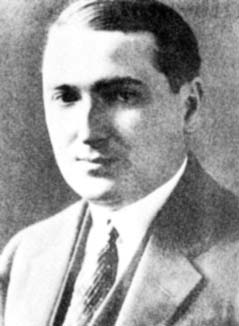
\includegraphics[width=2cm]{images/Post}

11.2.1897 -- 21.4.1954
\bigskip

Tragisches Genie\\
Wegbereiter der Logik\\
Stiller Vordenker von Gödel und Turing

\end{center}

\end{frame}

\begin{frame}\frametitle{Das Postsche Korrespondenzproblem}

\defbox{Das \redalert{Postsche Korrespondenzproblem} (PCP) besteht in der folgenden Frage.\\[1ex]
\emph{Gegeben:} eine endliche Folge von Wortpaaren\\[1ex]
% \narrowcentering{$\tuple{x_1,y_1}, \ldots, \tuple{x_k,y_k}$}\\[1ex]
\narrowcentering{$\left[\begin{matrix}x_1\\y_1\end{matrix}\right]\quad\ldots\quad\left[\begin{matrix}x_k\\y_k\end{matrix}\right]$}\\[1ex]
über einem Alphabet $\Sigma^*$.\\[1ex]
\emph{Frage:} Gibt es eine Folge von Zahlen $i_1,\ldots,i_\ell$, so dass gilt\\[1ex]
\narrowcentering{$x_{i_1} \cdots x_{i_l} = y_{i_1} \cdots y_{i_l}$,}\\[1ex]
wobei $\ell>0$ ist und $i_j\in\{1,\ldots,k\}$ für alle $j=1,\ldots,\ell$?
}

\end{frame}

\begin{frame}\frametitle{Beispiele}

 \[
\left[\begin{matrix}\Sterm{AB}\\\Sterm{B}\end{matrix}\right]\quad
\left[\begin{matrix}\Sterm{B}\\\Sterm{BBB}\end{matrix}\right]\quad
\left[\begin{matrix}\Sterm{BB}\\\Sterm{BA}\end{matrix}\right]
 \]

 \pause Dieses PCP hat eine Lösung mit 10 Schritten (Bonusaufgabe).\pause

\bigskip
\[
\left[\begin{matrix}\Sterm{ABB}\\\Sterm{A}\end{matrix}\right]\quad
\left[\begin{matrix}\Sterm{BB}\\\Sterm{AAB}\end{matrix}\right]\quad
\left[\begin{matrix}\Sterm{A}\\\Sterm{BB}\end{matrix}\right]\quad
\left[\begin{matrix}\Sterm{A}\\\Sterm{BAA}\end{matrix}\right]
 \] 
\pause Dieses PCP hat ebenfalls eine Lösung, aber keine mit weniger als 160 Schritten!\pause

\bigskip
\[
\left[\begin{matrix}\Sterm{AA}\\\Sterm{B}\end{matrix}\right]\quad
\left[\begin{matrix}\Sterm{BA}\\\Sterm{BAA}\end{matrix}\right]\quad
\left[\begin{matrix}\Sterm{ABA}\\\Sterm{A}\end{matrix}\right]
 \]
\pause Dieses PCP hat keine Lösung (Bonusaufgabe: Warum?).

\end{frame}

\begin{frame}\frametitle{Unentscheidbarkeit}

\theobox{Satz: Das PCP ist unentscheidbar.}\pause

Das zu zeigen ist nicht ganz so einfach, da das PCP auf den ersten Blick
nichts mit den uns bisher bekannten unentscheidbaren Problemen zu tun hat.
\bigskip

Wir gehen in zwei Schritten vor:
\begin{enumerate}[(1)]
\item Wir reduzieren das Halteproblem auf ein \alert{modifiziertes PCP}
\item Wir reduzieren das modifizierte PCP auf PCP
\end{enumerate}\bigskip\pause

\defbox{Eine Instanz des \redalert{Modifizierten PCP} (MPCP) ist eine Instanz des PCP (d.h. eine Menge von Wortpaaren), für die ein bestimmtes Startpaar angegeben ist.
Die Lösung des MPCP ist eine Lösung des PCP, welche mit dem Startpaar beginnt.}

\end{frame}

\begin{frame}\frametitle{Turingmaschinen simulieren in MPCP (1)}

Wir wollen das Halteproblem von DTMs auf das MPCP reduzieren.\medskip

Wir entwickeln dazu eine \alert{Many-One-Reduktion}, die eine Instanz des Halteproblems
in eine Instanz des MPCP verwandelt.\\
$\leadsto$ Kodiere TM-Berechnungen als Sequenz von Wortpaaren
\bigskip\pause

\emph{Ansatz für die Reduktion:}
\begin{itemize}
\item Das Wort, welches zur Lösung des MPCP entsteht, kodiert den Lauf einer TM
\begin{itemize}
\item Hält die TM, dann ist er Lauf endlich und es gibt eine Lösung
\item Hält die TM nicht, dann wird es keine Lösung geben
\end{itemize}
\item Eine TM-Konfiguration können wir wie immer als Wort der Form $v\, q\, w$ darstellen
\item Wir kodieren einen Lauf als Folge von Konfigurationen, getrennt mit $\Sterm{\#}$ (kein Alphabetszeichen oder Zustand der TM)
\end{itemize}

\end{frame}

\begin{frame}\frametitle{Turingmaschinen simulieren in MPCP (2)}

Wie kann man sicherstellen, dass die MPCP-Lösung eine korrekte Folge von TM-Konfigurationen kodiert?\bigskip\pause

\emph{Kernidee:}
\begin{itemize}
\item Das Lösungswort soll wie folgt beginnen: $\Sterm{\#}c_0\Sterm{\#}c_1\Sterm{\#}c_3\Sterm{\#}\ldots$, wobei $c_i$ Konfigurationen kodieren
\item Beim PCP entsteht das Lösungswort doppelt, oben und unten
\item Wir beginnen mit $\left[\begin{matrix}\Sterm{\#}\\\Sterm{\#}c_0\Sterm{\#}\end{matrix}\right]$, d.h. das obere Wort liegt eine Konfiguration zurück
\item Wir definieren die Wortpaare so, dass man oben eine Kopie der unteren Konfiguration nur dann erzeugen kann, wenn man gleichzeitig unten die Nachfolgerkonfiguration anfügt
\item Falls die TM hält, dann sorgen wir dafür, dass das obere Wort die fehlende Konfiguration aufholen kann
\end{itemize}

\end{frame}

\begin{frame}\frametitle{Turingmaschinen simulieren in MPCP (3)}

\alert{Überführungsregeln} kodieren die Übergänge der DTM:

\begin{align*}
\left[\begin{matrix}q\Sterm{a}\\\Sterm{b}p\end{matrix}\right]\quad
	& \text{falls $\delta(q,\Sterm{a})=\tuple{p,\Sterm{b},R}$}\\
\left[\begin{matrix}\Sterm{c}q\Sterm{a}\\p\Sterm{cb}\end{matrix}\right]\quad
	& \text{falls $\delta(q,\Sterm{a})=\tuple{p,\Sterm{b},L}$ und $\Sterm{c}\in\Gamma$ beliebig}\\
\left[\begin{matrix}q\Sterm{a}\\p\Sterm{b}\end{matrix}\right]\quad
	& \text{falls $\delta(q,\Sterm{a})=\tuple{p,\Sterm{b},N}$}
\end{align*}

In diesen Regeln steckt die Kernidee des Beweises. Es sind die wesentlichen Regeln, mit denen man Zustandssymbol $q\in Q$ im oberen Wort replizieren kann.

\end{frame}

\begin{frame}\frametitle{Turingmaschinen simulieren in MPCP (4)}

Es gibt zwei \alert{Randfälle:}\bigskip

Am linken Rand soll unsere TM einfach "`anstoßen"' (einseitig unendliches Band):
\begin{align*}
\left[\begin{matrix}\Sterm{\#}q\Sterm{a}\\\Sterm{\#}p\Sterm{b}\end{matrix}\right]\quad
	& \text{falls $\delta(q,\Sterm{a})=\tuple{p,\Sterm{b},L}$}
\end{align*}

Am rechten Rand kann die TM das Band beliebig erweitern:

\begin{align*}
\left[\begin{matrix}q\Sterm{\#}\\q\blank\Sterm{\#}\end{matrix}\right]\quad
	& \text{für jeden Zustand $q\in Q$}
\end{align*}

\textcolor{devilscss}{Anmerkung: Diese Umformung ist kein echter Rechenschritt, aber erspart uns die Auflistung von Sonderfällen für jede denkbare Transition am rechten Rand.}

\end{frame}

\begin{frame}\frametitle{Turingmaschinen simulieren in MPCP (5)}

\alert{Kopierregeln} erlauben uns, den Rest der TM-Konfiguration (die Teile, die nicht nah am Lese-/Schreibkopf liegen) vom unteren zum oberen Wort zu kopieren:

\begin{align*}
\left[\begin{matrix}x\\ x\end{matrix}\right]\quad
	& \text{für jedes Symbol $x\in \Gamma\cup\{\Sterm{\#}\}$}
\end{align*}

\textcolor{devilscss}{Anmerkung: Damit kann man keine Zustände kopieren.}
\bigskip\pause

Die \alert{Startregel} schließlich setzt die Berechnung in Gang:

\begin{align*}
\left[\begin{matrix}\Sterm{\#}\\ \Sterm{\#}q_0 w\Sterm{\#}\end{matrix}\right]\quad
	& \text{wobei $q_0$ der Startzustand und $w\in\Sigma^*$ das Eingabewort ist}
\end{align*}

\end{frame}

\begin{frame}\frametitle{Turingmaschinen simulieren in MPCP (6)}

\emph{Zwischenstand:} angefangen von der Startregel zwingen uns die Regeln, Konfigurationen
zu kopieren und dabei entweder einen Berechnungsschritt auszuführen, oder mehr Speicher am
rechten Rand zu allozieren.
\bigskip\pause

Es fehlt noch ein \alert{Abschluss:}\\
{(wir verwenden ein weiteres zusätzliches Symbol $\medbullet$)}

\begin{align*}
\left[\begin{matrix}q\Sterm{a}\\\medbullet\end{matrix}\right]\quad
	& \text{falls $\delta(q,\Sterm{a})$ undefiniert und $a\in\Gamma$ (d.h. $a\neq\Sterm{\#}$)}\\
\left[\begin{matrix}\Sterm{a}\medbullet\\\medbullet\end{matrix}\right]\quad\text{und}\quad\left[\begin{matrix}\medbullet\Sterm{a}\\\medbullet\end{matrix}\right]\quad
	& \text{für alle $\Sterm{a}\in\Gamma$}\\
% \left[\begin{matrix}\Sterm{a}\medbullet\\\medbullet\end{matrix}\right]\quad
% 	& \text{für alle $\Sterm{a}\in\Gamma$ beliebig}\\
\left[\begin{matrix}\medbullet\Sterm{\#}\Sterm{\#}\\\Sterm{\#}\end{matrix}\right]\quad
	& \text{der endgültige Abschluss}
\end{align*}

\end{frame}

\begin{frame}\frametitle{Turingmaschinen simulieren in MPCP (7)}

\theobox{Satz: Es gibt eine Many-One-Reduktion vom Halteproblem auf das
modifizierte PCP.}

\emph{Beweis:} Wir haben die Reduktion gerade angegeben, wobei das Wortpaar
mit der Startkonfiguration das Startpaar des MPCP ist.
\bigskip

Korrektheit (Skizze):
\begin{itemize}
\item Wenn es einen haltenden Lauf gibt, dann kann man eine Lösung des MPCP finden: gemäß Konstruktion
\item Wenn es eine Lösung für das MPCP gibt, dann hält die TM:
	\begin{itemize}
	\item Wir können die Übergänge als Berechnungsschritte interpretieren, d.h. es entsteht ein Lauf
	\item Das obere Wort ist anfangs kürzer und wird in keiner Regel länger als das untere, solange nicht eine haltende Konfiguration erreicht wurde
	\item Also kann das MPCP nur dann eine Lösung haben, wenn die TM hält.\qed
	\end{itemize}
\end{itemize}

\end{frame}

\begin{frame}[t]\frametitle{Von PCP zu MPCP (1)}

Es fehlt noch eine Reduktion von MPCP auf PCP.\bigskip

\theobox{Satz: Es gibt eine Many-One-Reduktion vom 
modifizierten PCP auf PCP.}

\emph{Beweis:} Wir verwenden zwei zusätzliche Symbole $\Sterm{\#}$ und 
$\Sterm{\blacksquare}$. Für ein Wort $w=a_1\cdots a_\ell$
definieren wir:
\begin{align*}
{}_{\Sterm{\#}}w_{\Sterm{\#}} &= \Sterm{\#}{a_1}\Sterm{\#}\cdots\Sterm{\#}{a_\ell}\Sterm{\#} &
w_{\Sterm{\#}} &= {a_1}\Sterm{\#}\cdots\Sterm{\#}{a_\ell}\Sterm{\#} &
{}_{\Sterm{\#}}w &= \Sterm{\#}{a_1}\Sterm{\#}\cdots\Sterm{\#}{a_\ell}
\end{align*}
Die gesuchte Reduktion bildet jetzt ein MPCP\\[1ex]
\narrowcentering{$\left[\begin{matrix}x_1\\y_1\end{matrix}\right]\quad\ldots\quad\left[\begin{matrix}x_k\\y_k\end{matrix}\right]$}\\[1ex]
ab auf das PCP\\[1ex]
\narrowcentering{$%
\left[\begin{matrix}{}_{\Sterm{\#}}x_1{}_{\Sterm{\#}}\\{}_{\Sterm{\#}}y_1\end{matrix}\right]
\quad\left[\begin{matrix}x_1{}_{\Sterm{\#}}\\{}_{\Sterm{\#}}y_1\end{matrix}\right]
\quad\ldots
\quad\left[\begin{matrix}x_k{}_{\Sterm{\#}}\\{}_{\Sterm{\#}}y_k\end{matrix}\right]
\quad\left[\begin{matrix}\Sterm{\blacksquare}\\\Sterm{\#\blacksquare}\end{matrix}\right]
$}\\[1ex]


\end{frame}

\begin{frame}[t]\frametitle{Von PCP zu MPCP (2)}

% Es fehlt noch eine Reduktion von MPCP auf PCP.\bigskip
% 
% \theobox{Satz: Es gibt eine Many-One-Reduktion vom 
% modifizierten PCP auf PCP.}

\emph{Beweis (Fortsetzung):} Wir erhalten also das folgende PCP\\[1ex]
\narrowcentering{$%
\left[\begin{matrix}{}_{\Sterm{\#}}x_1{}_{\Sterm{\#}}\\{}_{\Sterm{\#}}y_1\end{matrix}\right]
\quad\left[\begin{matrix}x_1{}_{\Sterm{\#}}\\{}_{\Sterm{\#}}y_1\end{matrix}\right]
\quad\ldots
\quad\left[\begin{matrix}x_k{}_{\Sterm{\#}}\\{}_{\Sterm{\#}}y_k\end{matrix}\right]
\quad\left[\begin{matrix}\Sterm{\blacksquare}\\\Sterm{\#\blacksquare}\end{matrix}\right]
$}\\[1ex]
%
Es ist nicht schwer zu zeigen, dass dies genau dann eine Lösung hat, wenn das ursprüngliche MPCP eine hat:\pause
\begin{itemize}
\item "`$\Leftarrow$"' Wenn das MPCP eine Lösung hat, dann erhalten wir leicht eine entsprechende Lösung für das PCP, wobei jedes Symbol zusätzlich von $\Sterm{\#}$ umgeben ist und das Wort auf $\Sterm{\blacksquare}$ endet\pause
\item "`$\Rightarrow$"' Wenn das PCP eine Lösung hat, dann muss es mit dem ersten Wortpaar beginnen, da nur dieses Wortpaar gleiche Anfangssymbole hat. Durch Weglassen aller $\Sterm{\#}$ und 
$\Sterm{\blacksquare}$ entsteht wieder eine Lösung des MPC.\qed
\end{itemize}

\end{frame}


\begin{frame}\frametitle{Zusammenfassung und Ausblick}

Alle interessanten Fragen über Turingmaschinen sind unentscheidbar\bigskip

\alert{Semi-Entscheidbarkeit} wird durch Many-One-Reduktionen erhalten, nicht aber durch Turing-Reduktionen\bigskip

Das \alert{Postsche Korrespondenzproblem} ist ein unentscheidbares Problem, das nicht (direkt) mit TMs zu tun hat -- es ist hilfreich bei vielen Reduktionen\bigskip

\anybox{yellow}{
Was erwartet uns als nächstes?
\begin{itemize}
\item Abschließende Bemerkungen zu Berechenbarkeit
\item Methoden, zur Unterteilung entscheidbarer Probleme: Komplexität
\end{itemize}
}

\end{frame}

\begin{frame}[t]\frametitle{Literatur und Bildrechte}

\alert{Literatur}\bigskip

\begin{itemize}
\item Richard J. Lorentz:
\emph{Creating Difficult Instances of the Post Correspondence Problem.}
Computers and Games 2000: 214--228
\item John J. O'Connor, Edmund F. Robertson: \emph{Emil Leon Post.} MacTutor History of Mathematics archive, University of St Andrews. \url{http://www-history.mcs.st-andrews.ac.uk/Biographies/Post.html}
\end{itemize}

\bigskip\bigskip

\alert{Bildrechte}\bigskip

Folie \ref{frame_post}: gemeinfrei

\end{frame}


\end{document}
